%% Direttive TeXworks:
% !TeX root = ../maltoni_niccolo_tesi.tex
% !TEX encoding = UTF-8 Unicode
% !TEX program = arara
% !TEX TS-program = arara
% !TeX spellcheck = it-IT

%% Direttive Arara:
% arara: pdflatex: { shell: yes, synctex: yes, action: batchmode, options: "-halt-on-error -file-line-error-style" }
% arara: frontespizio
% arara: biber
% arara: pdflatex: { shell: yes, synctex: yes, action: batchmode, options: "-halt-on-error -file-line-error-style" }
% arara: pdflatex: { shell: yes, synctex: yes, action: nonstopmode, options: "-halt-on-error -file-line-error-style" }

\chapter{Contributo}\label{ch:contributo}
    In questo capitolo verrà analizzato il contributo fornito al progetto, elencando i requisiti necessari e analizzando il processo di soddisfazione degli stessi.

    L'obiettivo principale è quello di integrare una nuova interfaccia per la simulazione, al fine di semplificare l’adozione del simulatore da parte di utenti inesperti.

    \section{Analisi dei requisiti}\label{sec:analisi}
        Lo studio del lavoro illustrato in questa tesi ha inizio con l'analisi dei requisiti dell’interfaccia utente, ossia cosa l'applicazione deve mostrare a schermo.

        Questa sezione si occuperà di enunciare i requisiti funzionali e non funzionali individuati.

        \subsection{Requisiti funzionali}\label{sub:funzionali}
            I requisiti funzionali (\figurename~\ref{fig:useCase}) descrivono il comportamento che il sistema deve avere:
            descrivono le funzionalità del sistema software, in termini di servizi che il sistema software deve fornire, di come il sistema software reagisce a specifici tipi di input e di come si comporta in situazioni particolari.

            \subsubsection{Rappresentazione dell'ambiente di simulazione}\label{subsub:seeEnv}
                Essendo la componente grafica da reimplementare quella legata alla simulazione in escuzione, requisito fondamentale è che la GUI possa rappresentare l'ambiente con le maggiori possibilità di dettaglio possibile.

                Di conseguenza, deve essere presente uno spazio disegnabile in cui si possa avere una rappresentazione grafica di quanto accade, ma anche contatori che mostrino l'avanzamento della simulazione in termini di tempo (secondi) trascorso e passaggi (\engEmph{step}) effettuati.

            \subsubsection{Gestione degli effetti}\label{subusub:manageEffects}
                La nuova interfaccia deve rendere possibile all'utente di poter aggiungere nuovi effetti allo \engEmph{stack} di rappresentazione e modificarne le proprietà a tempo di esecuzione.

                Inoltre attraverso la GUI l'utente deve poter salvare lo stack di effetti presente in quel momento e caricarlo in un secondo momento, mantenendo tutte le proprietà definite manualmente.

                Infine, deve essere possibile nascondere singoli effetti o gruppi di essi senza rimuoverli dallo \engEmph{stack}.

            \subsubsection{Effetti standard per nodi e collegamenti}\label{subusub:defaultEffects}
                Devono essere implementati effetti adibiti alla rappresentazione dei singoli nodi come punti e dei collegamenti tra i nodi di un vicinato.

                Questi effetti dovranno essere caricati automaticamente al lancio dell'applicazione, salvo diversamente specificato.

            \subsubsection{Interazione con simulazione e ambiente rappresentato}\label{subsub:interazione}
                L'interfaccia deve mettere a disposizione dell'utente la capacità di interagire con la simulazione, potendo fermarla e riavviarla, interagire con i nodi e spostarsi tra essi. Deve essere possibile effettuare pan e zoom sull'ambiente rappresentato.

                Le possibilità di interazione non devono essere vincolate al puntatore del mouse, ma deve supportare anche le scorciatoie da tastiera.

            \subsubsection{Rappresentazione di ambienti con mappa}\label{subsub:mappa}
                Deve essere fornito il supporto alle mappe come sfondo degli ambienti nella rappresentazione di simulazioni che coinvolgano questo aspetto.

                \begin{figure}[htbp]
                    \centering
                    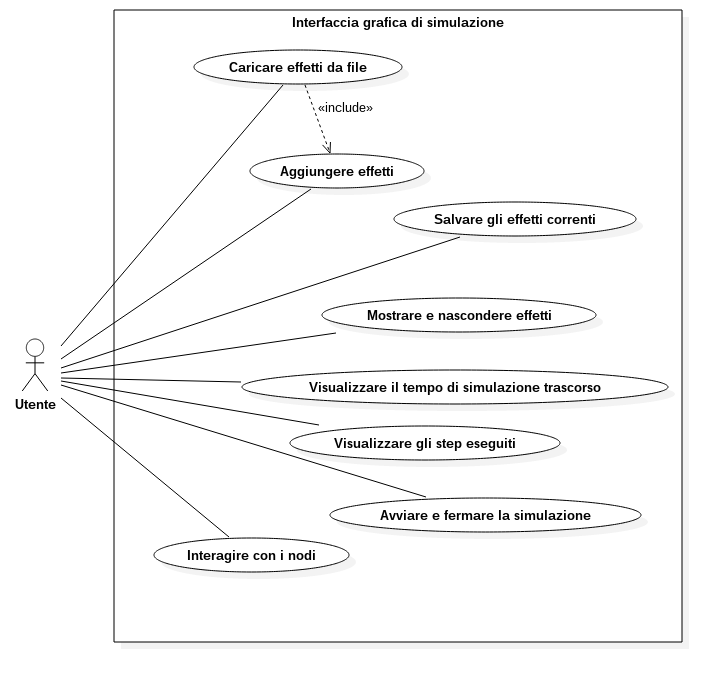
\includegraphics[scale=0.55]{img/useCase}
                    \caption{Requisiti funzionali principali}
                    \label{fig:useCase}
                \end{figure}

        \subsection{Requisiti non funzionali}\label{sub:nonFunzionali}
            I requisiti non funzionali descrivono le proprietà non comportamentali che il sistema deve possedere, come efficienza, affidabilità, sicurezza, performance, ma anche caratteristiche del processo di sviluppo e caratteristiche esterne.

            \subsubsection{JavaFX}\label{subsub:jfx}
                Come specificato nella sezione~\vref{sec:motivi}, il processo di sviluppo deve coinvolgere la libreria JavaFX come framework per la costruzione dell'interfaccia.

            \subsubsection{Performance}\label{subsub:performance}
                L'interfaccia grafica deve quanto più possibile non gravare sulle prestazioni del motore di simulazione; in particolare, poiché JavaFX non è nativamente \engEmph{thread-safe}, è necessario gestire la concorrenza in modo oculato.

            \subsubsection{Supporto Hi-DPI}\label{subsub:hidpi}
                L'interfaccia non deve perdere di usabilità e qualità di rappresentazione su alcun tipo di schermo, indipendentemente dalla risoluzione e dalla densità di pixel.Per fare questo si devono quindi utilizzare quanto più possibile grandezze relative e sfruttare al meglio in tal senso le funzionalità offerte da JavaFX.

    \section{Fonti d'ispirazione}\label{sec:ispirazione}


        \subsection{Simulatori a scopo videoludico}\label{sub:videogame}
            \subsubsection{Universe Sandbox}\label{subsub:us1}
            \subsubsection{Universe Sandbox 2}\label{subsub:us2}
            \subsubsection{SimCity}\label{subsub:simcity}
        \subsection{Material Design}\label{sub:material}
    \section{Design dell'interfaccia}\label{sec:design}
    \section{Progettazione}\label{sec:progettazione}
        \subsection{La barra inferiore}\label{sub:barra}
        \subsection{La struttura a drawer}\label{sub:drawer}
        \subsection{L'architettura degli effetti}\label{sub:effetti}
            % \subsubsection{I gruppi di effetti e l'interfaccia \texttt{EffectGroup}}\label{subsub:effectGroup}
            % \subsubsection{I singoli effetti e l'interfaccia \texttt{EffectFX}}\label{subsub:effectFX}
            % \subsubsection{Caricamento, salvataggio e modifica di gruppi di effetti}\label{subsub:serializzazione}
    \section{Dettagli implementativi}\label{sec:dettagli}
        % \subsection{Librerie utilizzate}\label{sub:lib}
        % \subsection{Gestione della concorrenza}\label{sub:concorrenza}
